\section{Плоская диаграмма}

Проекция узла в регулярном положении с указанием проходов и переходов - называется плоской диаграммой узла.
Проекция узла в регулярном положении без указания проходов и переходов - называется тенью узла. 

Плоская диаграмма и тень узла являются четырёхвалентными графами.

Над плоской диаграммой определены движения Рейдемейстера, которые являются эквивалентными преобразованиями.

\paragraph{Теорема (Рейдемейстер)} Две плоские диаграммы $D_1$ и $D_2$ порождают эквивалентные узлы тогда и только тогда, когда $D_1$ может быть преобразована в $D_2$ движениями Рейдемейстера.



\graphicspath{{\currentpath}}

$\Omega_1$ - закручивание и раскручивание колышки

\begin{tabular}{
>{\centering\arraybackslash}m{3cm}>{\centering\arraybackslash}m{0.4cm}
>{\centering\arraybackslash}m{3cm}>{\centering\arraybackslash}m{0.4cm}
>{\centering\arraybackslash}m{3cm}
}
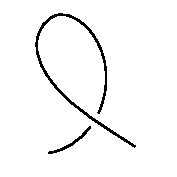
\includegraphics{images/close-loop-l.pdf}
&
=
&
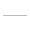
\includegraphics{images/line.pdf}
&
=
&
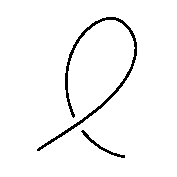
\includegraphics{images/close-loop-r.pdf}
\end{tabular}

$\Omega_2$ - занос одной линии петлёй над другой линией

\begin{tabular}{
>{\centering\arraybackslash}m{3cm}>{\centering\arraybackslash}m{0.4cm}
>{\centering\arraybackslash}m{3cm}>{\centering\arraybackslash}m{0.4cm}
>{\centering\arraybackslash}m{3cm}
}
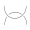
\includegraphics{images/two-loops-up.pdf}
&
=
&
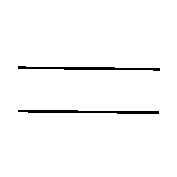
\includegraphics{images/two-line.pdf}
&
=
&
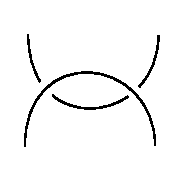
\includegraphics{images/two-loops-down.pdf}
\end{tabular}


$\Omega_3$ - если одна линия переходит над двумя другими, и они пересекаются недалеко от этой линии (другие линии не мешают картине), то первую линию можно расположить по другую сторону от пересечения других двух.

\begin{tabular}{
>{\centering\arraybackslash}m{3cm}>{\centering\arraybackslash}m{0.4cm}
>{\centering\arraybackslash}m{3cm}
}
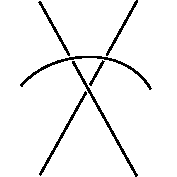
\includegraphics{images/over-cross-top.pdf}
&
=
&
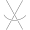
\includegraphics{images/over-cross-bottom.pdf}

\end{tabular}
